\documentclass[pdf, hyperref={unicode}, aspectratio=169]{beamer}

\usepackage{./diploma-slides-latex-template/styles}

% Включаю кнопочки
\setbeamertemplate{navigation symbols}[default]

% Название темы слишком длинное, поменьше шрифт!
\setbeamerfont{title}{series=\bfseries, size=\large}
\setbeamerfont{footline}{series=\bfseries, size=\fontsize{5}{3}\selectfont}

\useoutertheme{miniframes}

\title{Проектирование системы переноса и генерации взаимосвязанных данных из производственной среды при тестировании образовательной платформы}

\subtitle{Выпускная квалификационная работа бакалавра}

\pdfstringdefDisableCommands{
\def\\{}
\def\,{}
\def\textbf#1{<#1>}
}

\author[Мезенин Олег Александрович]
{
	\textbf{Студент группы М8О-406Б-21:} Мезенин Олег Александрович\\
	\ \textbf{Научный руководитель:} ст. преподаватель кафедры 806\\\ Миронов Евгений Сергеевич
	% Обратите внимание на пробел в начале строки
}

\institute[Московский авиационный институт]
{
	Московский авиационный институт (национальный исследовательский университет)\\
	Институт № 8 «Компьютерные науки и прикладная математика»\\
	Кафедра № 806 «Вычислительная математика и программирование» 
}

\date{Москва --- \the\year}

\logo{
\includegraphics[height=1cm]{img/mai}}


\begin{document}

\epstopdfsetup{outdir=./}

{
	% убирает номер слайда с титульного слайда
	\setbeamertemplate{page number in head/foot}{}
	\frame{\titlepage}
}

\begin{frame}
	\frametitle{Актуальность темы}
	\begin{itemize}
		\item Тестирование программного продукта является важной частью разработки.

		\item Тестирование в производственной среде сопряжено с рисками:
		\begin{itemize}
			\item нагрузка на систему;
			\item целостность данных;
			\item конфиденциальность данных.
		\end{itemize}

		\item Копирование всех данных (например, с помощью pg\_dump):
		\begin{itemize}
			\item занимает много времени;
			\item использует много ресурсов;
			\item не решается вопрос конфиденциальности данных.
		\end{itemize}

		\item Часто для тестовых сценариев нужны не все данные, а определённое количество согласованных данных.
	\end{itemize}
\end{frame}


\begin{frame}
	\frametitle{Цель и задачи работы}
	
	\textbf{Цель} --- проектирование системы, способной переносить взаимосвязанные данные, анонимизировать их и генерировать тестовые данные.

	\textbf{Задачи:}
	\begin{enumerate}
		\item определение требований;
		\item анализ аналогов;
		\item проектирование архитектуры;
		\item разработка алгоритмов переноса и генерации;
		\item разработка языка для описания данных;
		\item реализация минимально жизнеспособного продукта;
		\item анализ результатов.
	\end{enumerate}
\end{frame}


\begin{frame}
\frametitle{Архитектура системы переноса и генерации данных}
	\begin{center}
		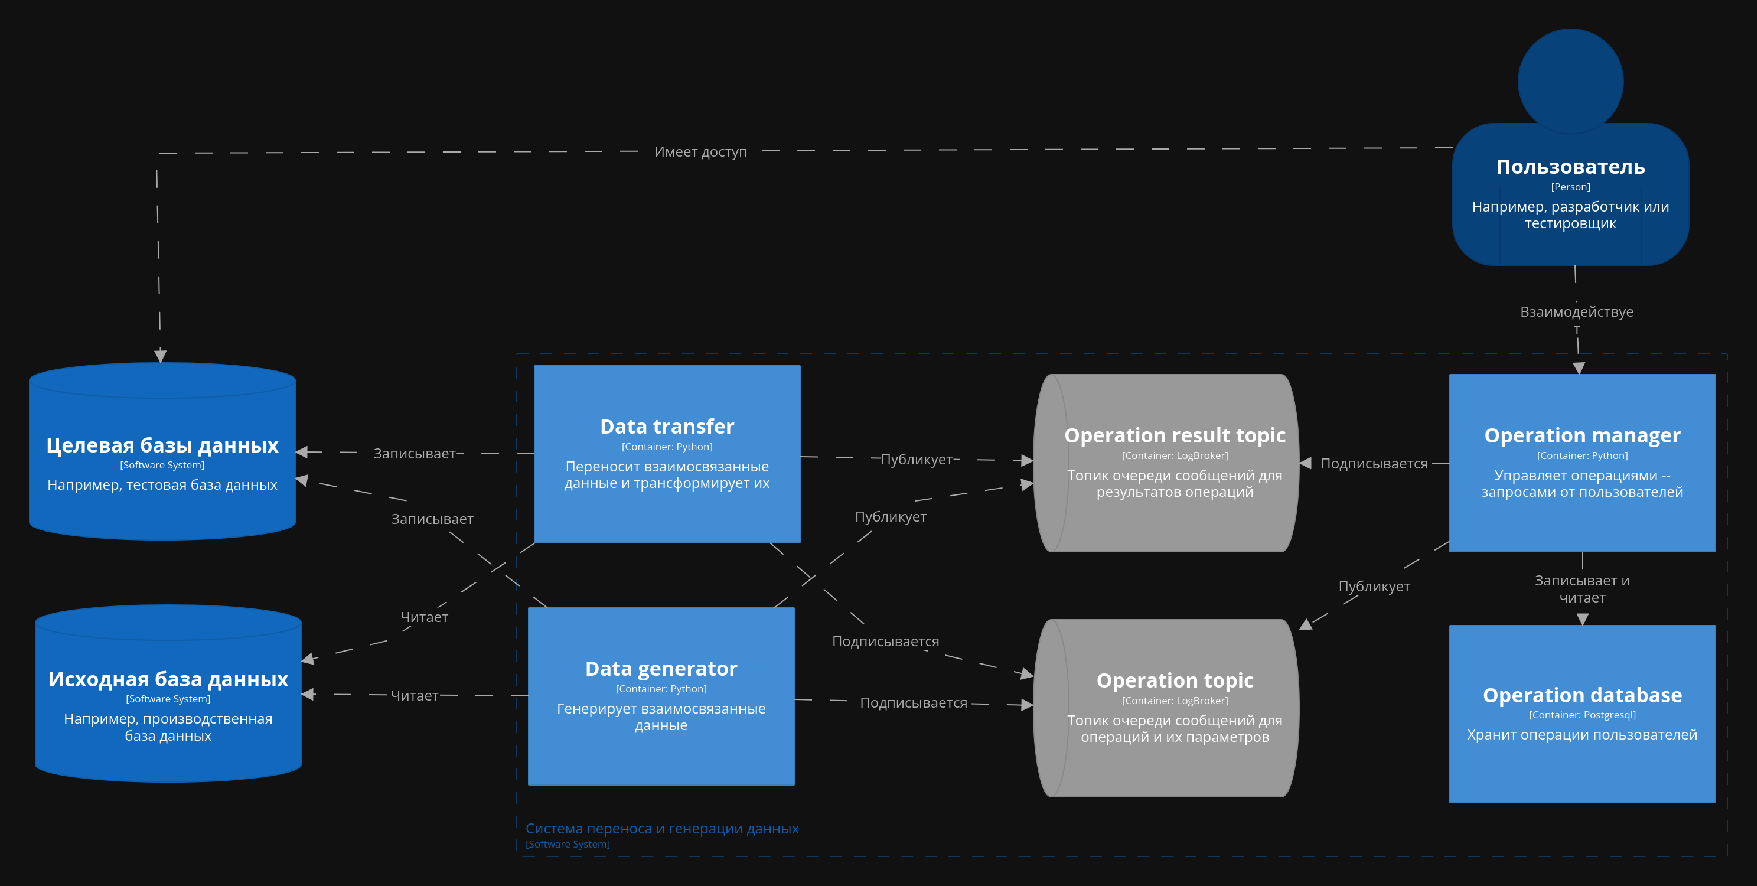
\includegraphics[height = 6.5cm]{img/structurizr-Containers-cut}
	\end{center}
\end{frame}


\begin{frame}
\frametitle{Архитектура Data Transfer}
	\begin{center}
		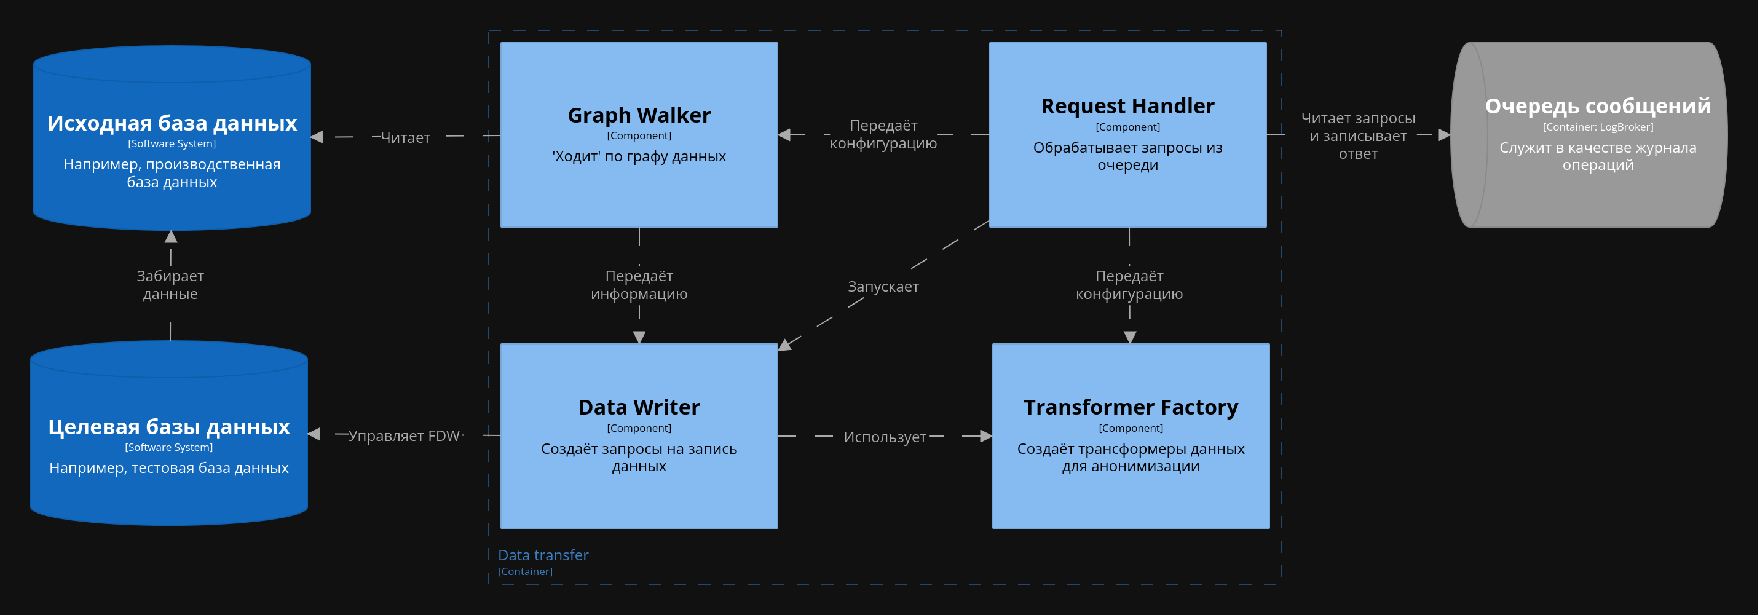
\includegraphics[width = 13cm]{img/structurizr-DataTransferComponents-cut}
	\end{center}
\end{frame}


\begin{frame}
\frametitle{Определение метаграфа}
	\textbf{Предпосылки} к использованию метаграфов:

	\begin{itemize}
		\item требовалось формализовать схему базы данных;
		\item классические графы и ER-модель не подходят ввиду ограниченных возможностей.
	\end{itemize}

	\textbf{Определение:} $MG = \langle V, MV, E, ME \rangle$ -- метаграф, где $V$ -- множество вершин, $MV$ -- множество метавершин, $E$ -- множество рёбер, $ME$ -- множество метарёбер.
\end{frame}


\begin{frame}
\frametitle{Соответствие метаграфа и базы данных}
	\begin{itemize}
		\item вершины $\Leftrightarrow$ записи;
		\item метавершины $\Leftrightarrow$ таблицы;
		\item рёбра $\Leftrightarrow$ связи между записями;
		\item метарёбра $\Leftrightarrow$ логические внешние ключи.
	\end{itemize}
\end{frame}


\begin{frame}
\frametitle{Пример базы данных}
	\begin{center}
		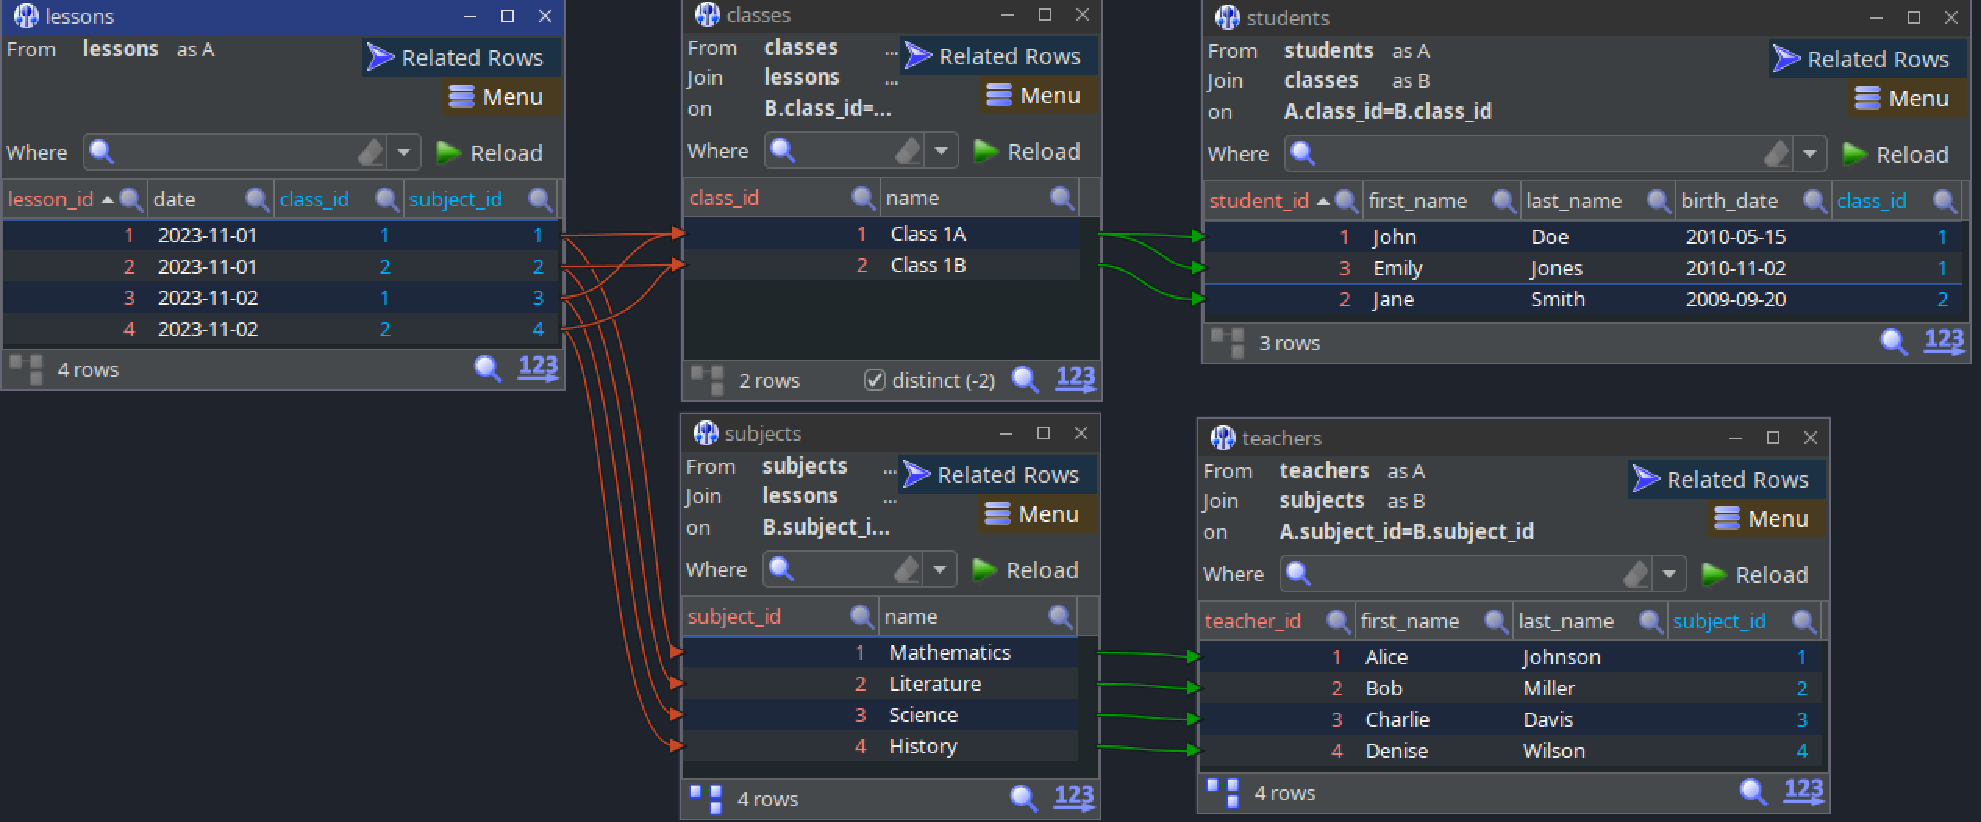
\includegraphics[width = 13cm]{img/jailer-example-db}
	\end{center}
\end{frame}


\begin{frame}
\frametitle{Графическое отображение метаграфа}
	\begin{center}
		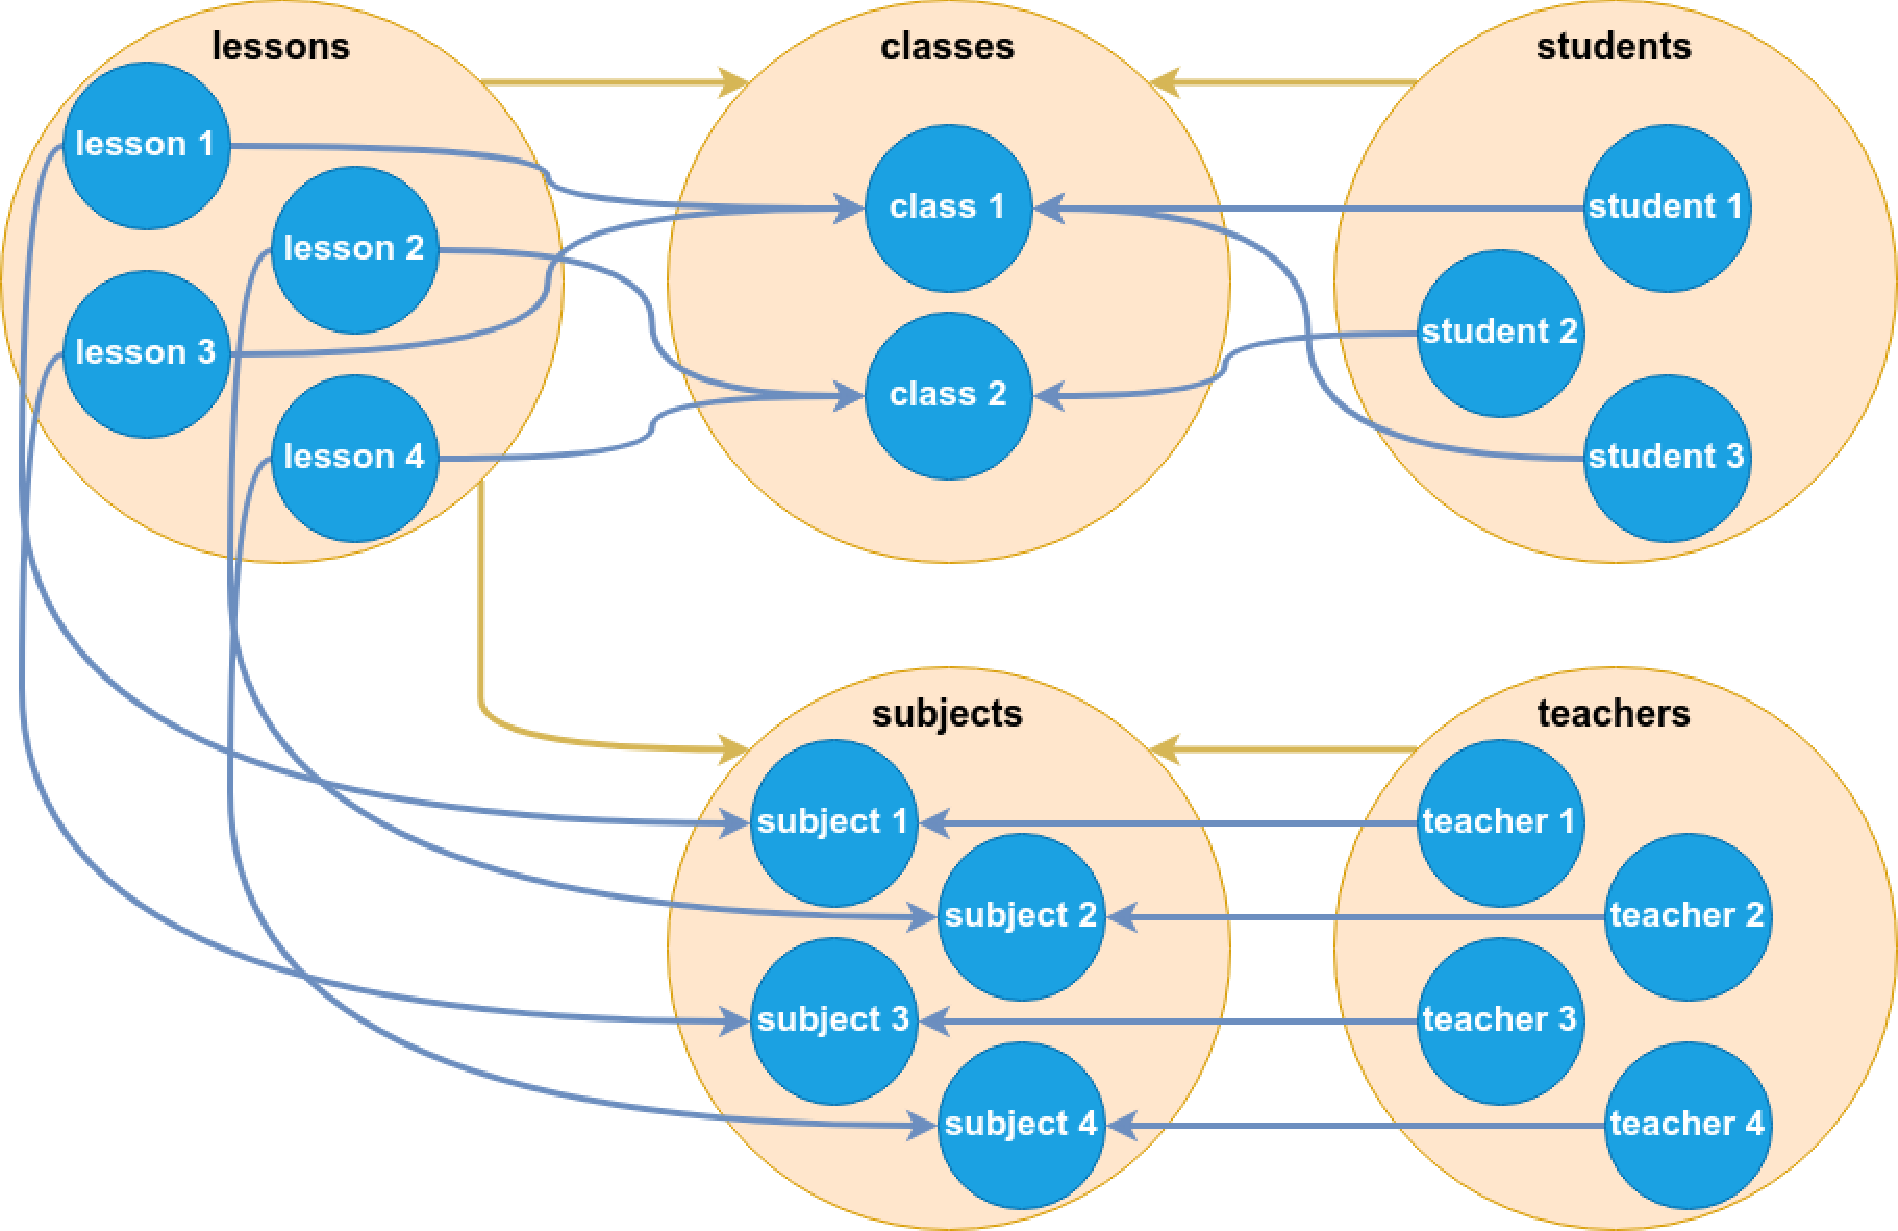
\includegraphics[height = 6.5cm]{img/drawio-metagraph}
	\end{center}
\end{frame}


\begin{frame}
\frametitle{Алгоритм обхода данных}

	\begin{center}
		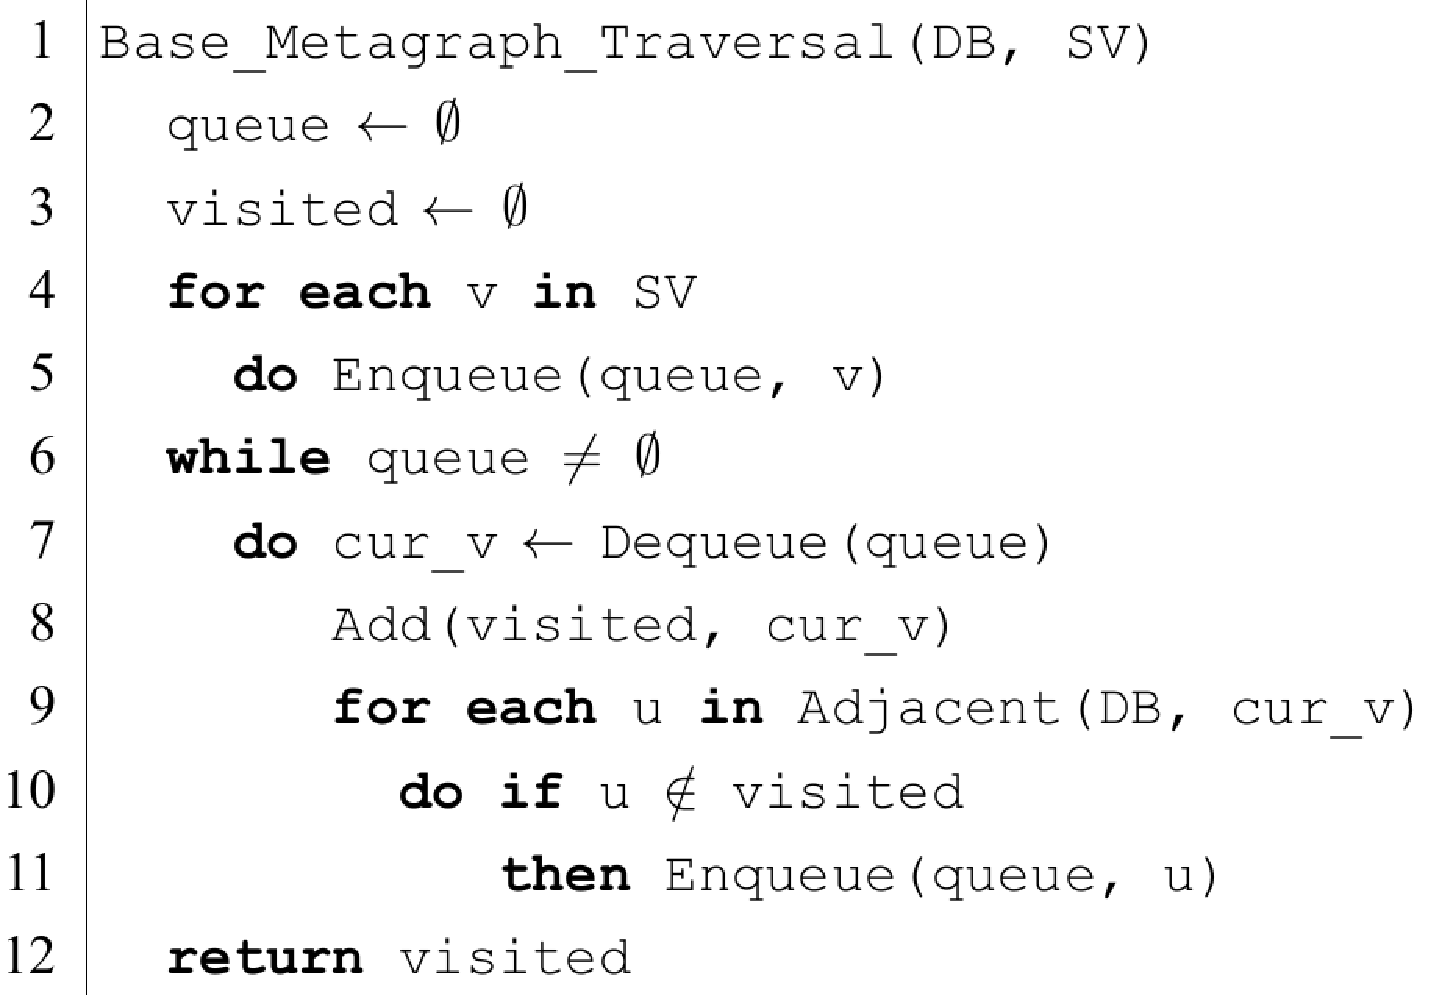
\includegraphics[height = 6.5cm]{img/algorithm-base}
	\end{center}
\end{frame}


\begin{frame}
\frametitle{Опреление правил метаграфа}
	\textbf{Предпосылки} к использованию правил метаграфа:
	\begin{itemize}
		\item изменение связей в метаграфе;
		\item ограничение обхода метаграфа.
	\end{itemize}

	\textbf{Определение:} $r = \langle p, f \rangle$ -- правило метаграфа, где $p$ — предикат, а $f$ — функция, изменяющая множество рёбер (метарёбер) метаграфа.

	$p: e => \{True, False\}$, где $e \in E$, $E$ -- множество рёбер (метарёбер).

	$f: E => E'$, где $E$ и $E'$ -- множество и обновлённое множество рёбер (метарёбер).
\end{frame}


\begin{frame}
\frametitle{Алгоритм обхода данных с правилами метаграфа}
	\begin{center}
		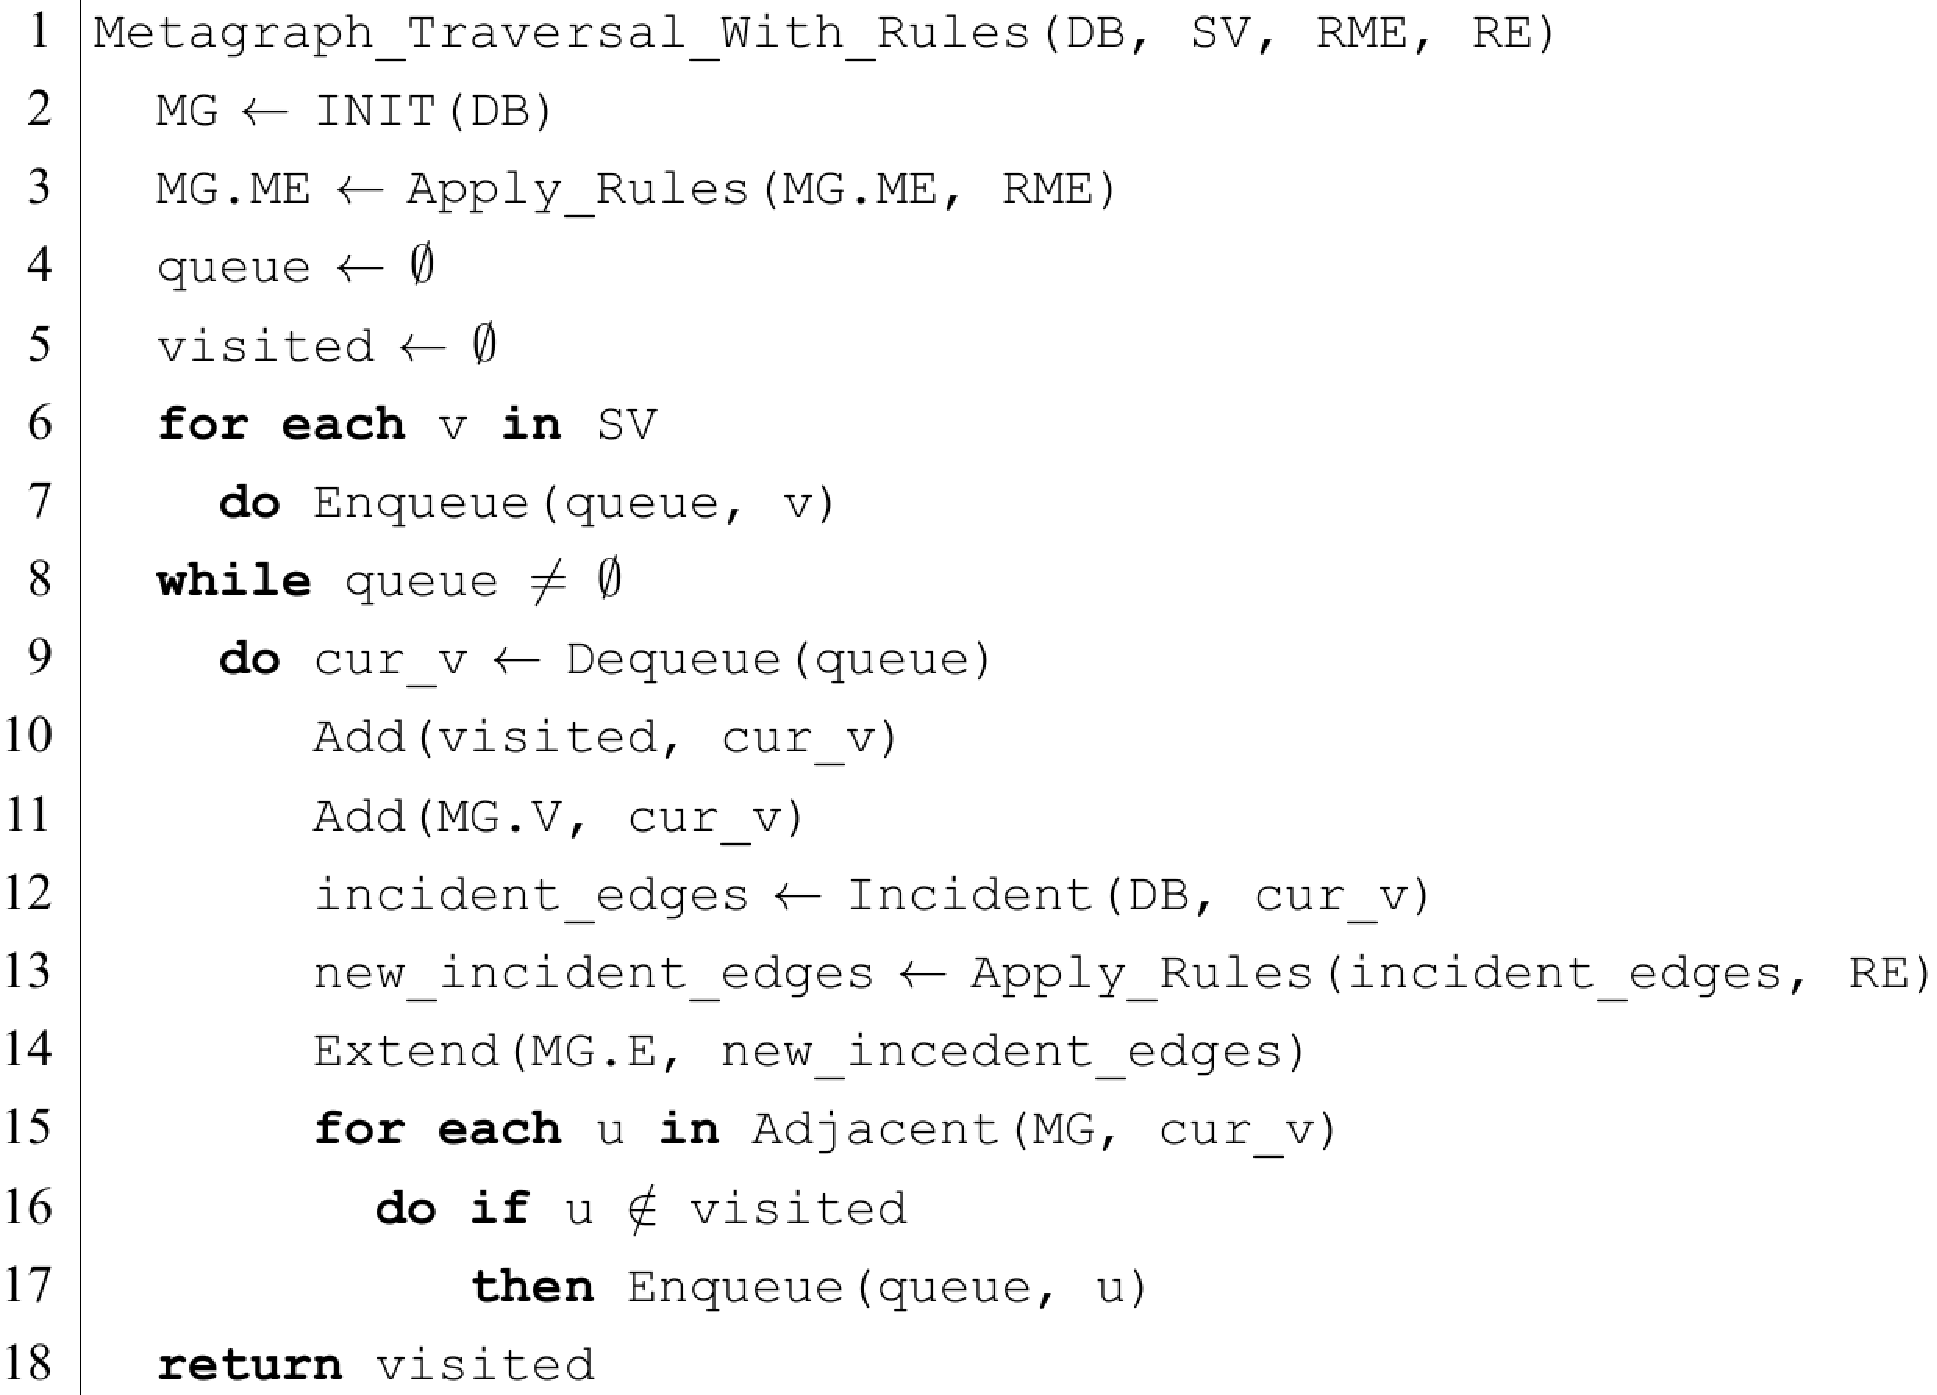
\includegraphics[height = 6.5cm]{img/algorithm-with-rules}
	\end{center}
\end{frame}


\begin{frame}
\frametitle{Язык описания обхода и трансформации данных}
	Разработан язык на основе грамматики SQL стандарта SQL-92 с помощью инструмента ANTLR4.
\end{frame}


\begin{frame}
\frametitle{Примеры грамматических конструкций на ANTLR4}
	\begin{center}
		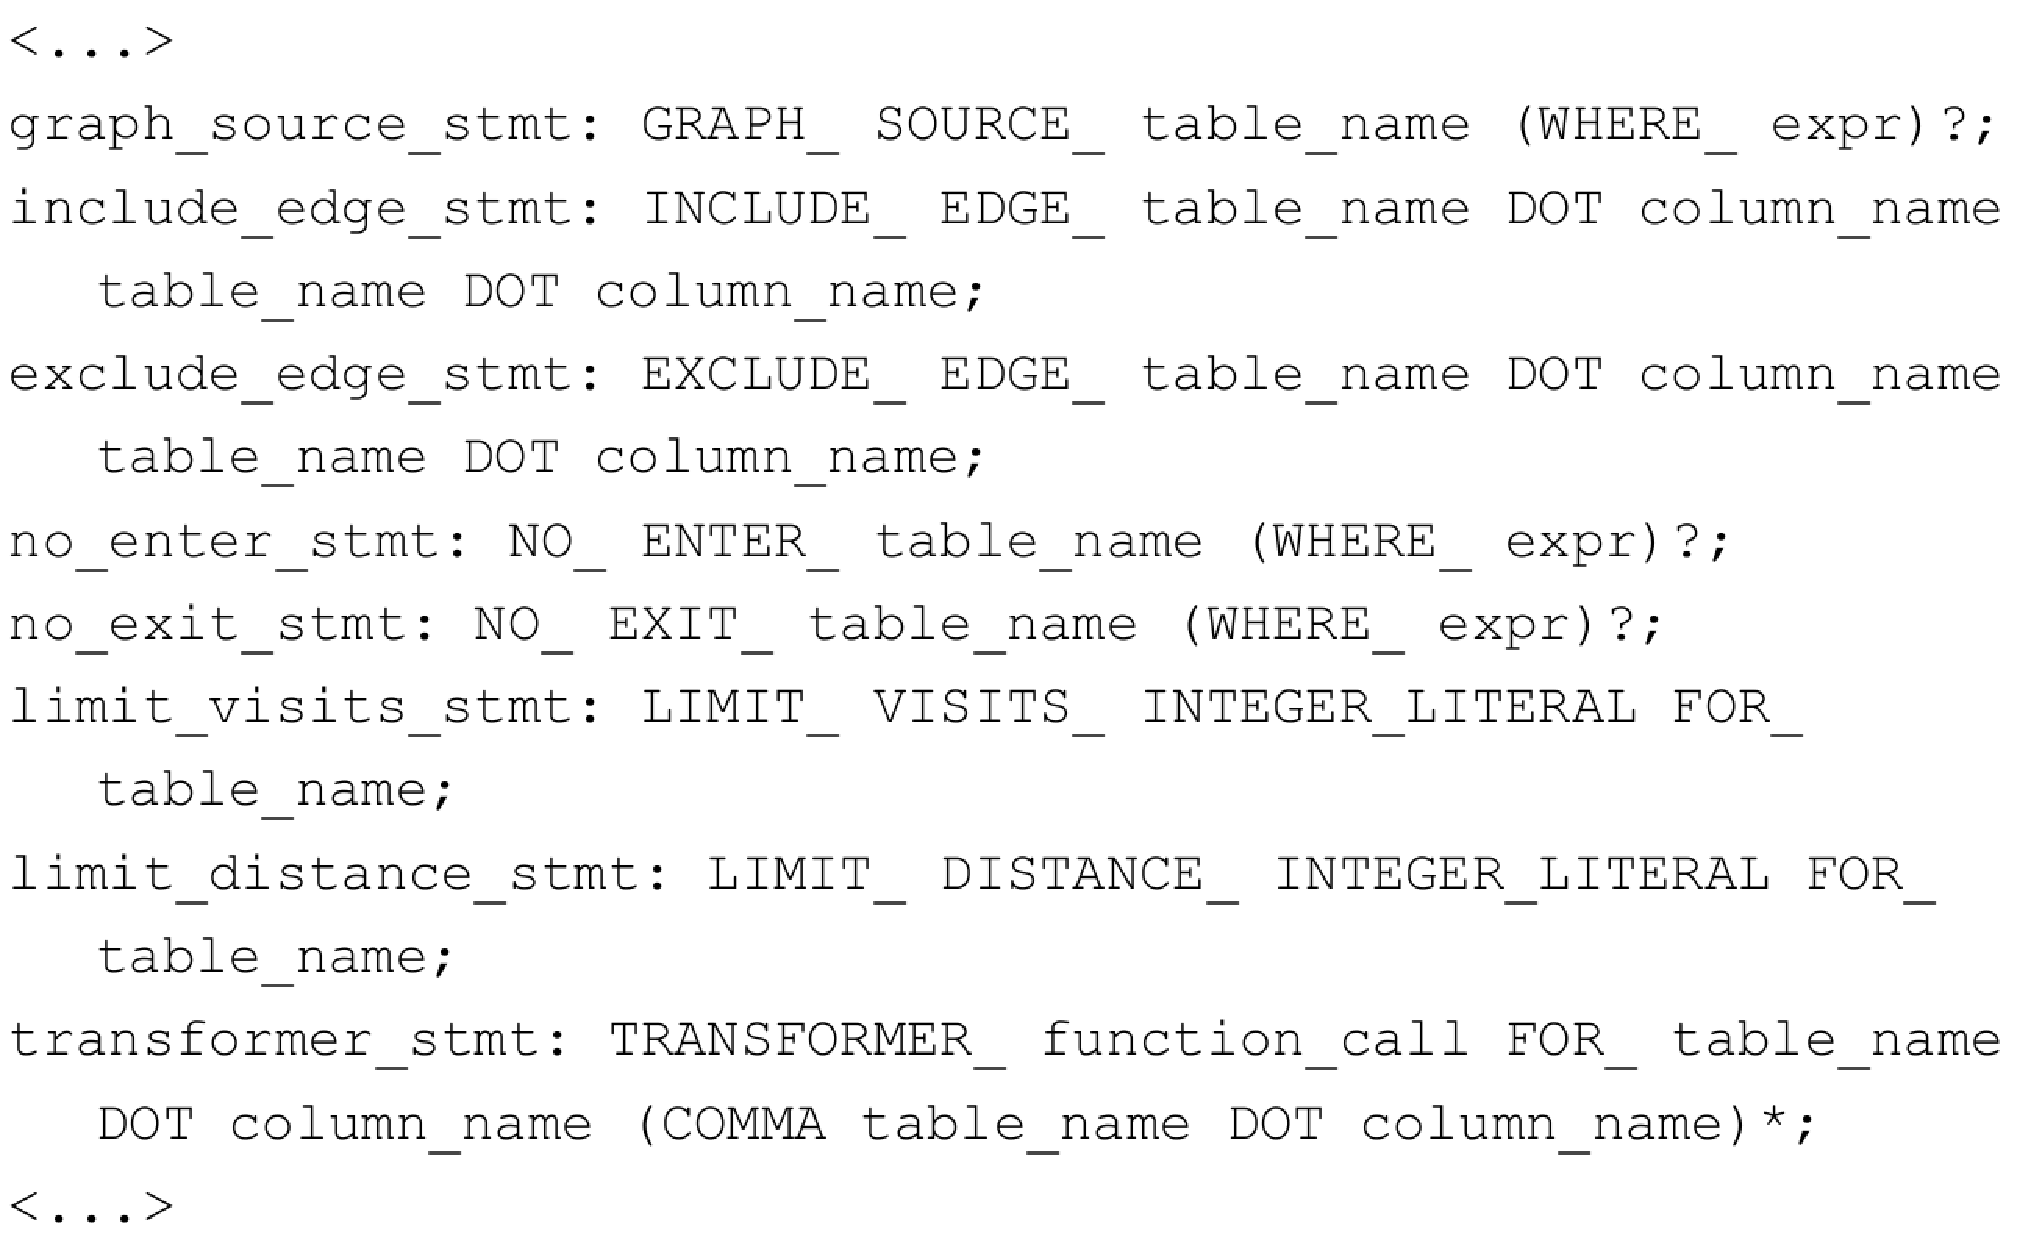
\includegraphics[height = 6.5cm]{img/grammar}
	\end{center}
\end{frame}


\begin{frame}
\frametitle{Пример описания обхода и трансформации данных}
	\begin{center}
		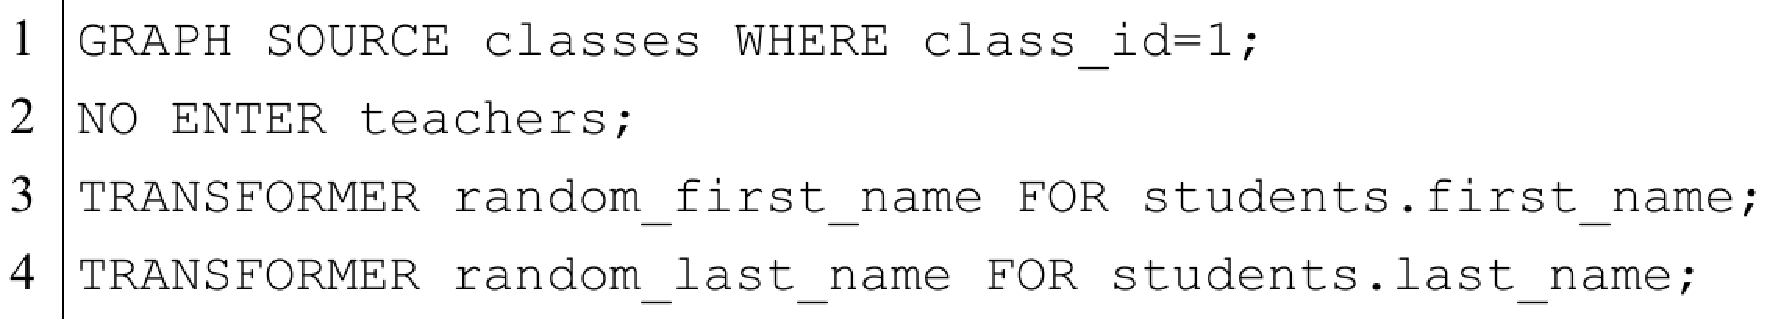
\includegraphics[width = 12cm]{img/language-1}
	\end{center}
\end{frame}


\begin{frame}
\frametitle{Минимально жизнеспособный продукт}
	\begin{itemize}
		\item интерфейс командной строки;
		\item перенос взаимосвязанных данных;
		\item построение метаграфа по базе данных;
		\item поддержка правил для ограничения обхода метаграфа.
	\end{itemize}
\end{frame}


\begin{frame}
\frametitle{Тесты производительности}
	Тестовая база данных: 4.5 ГБ, 44739072 записей

	\begin{center}
		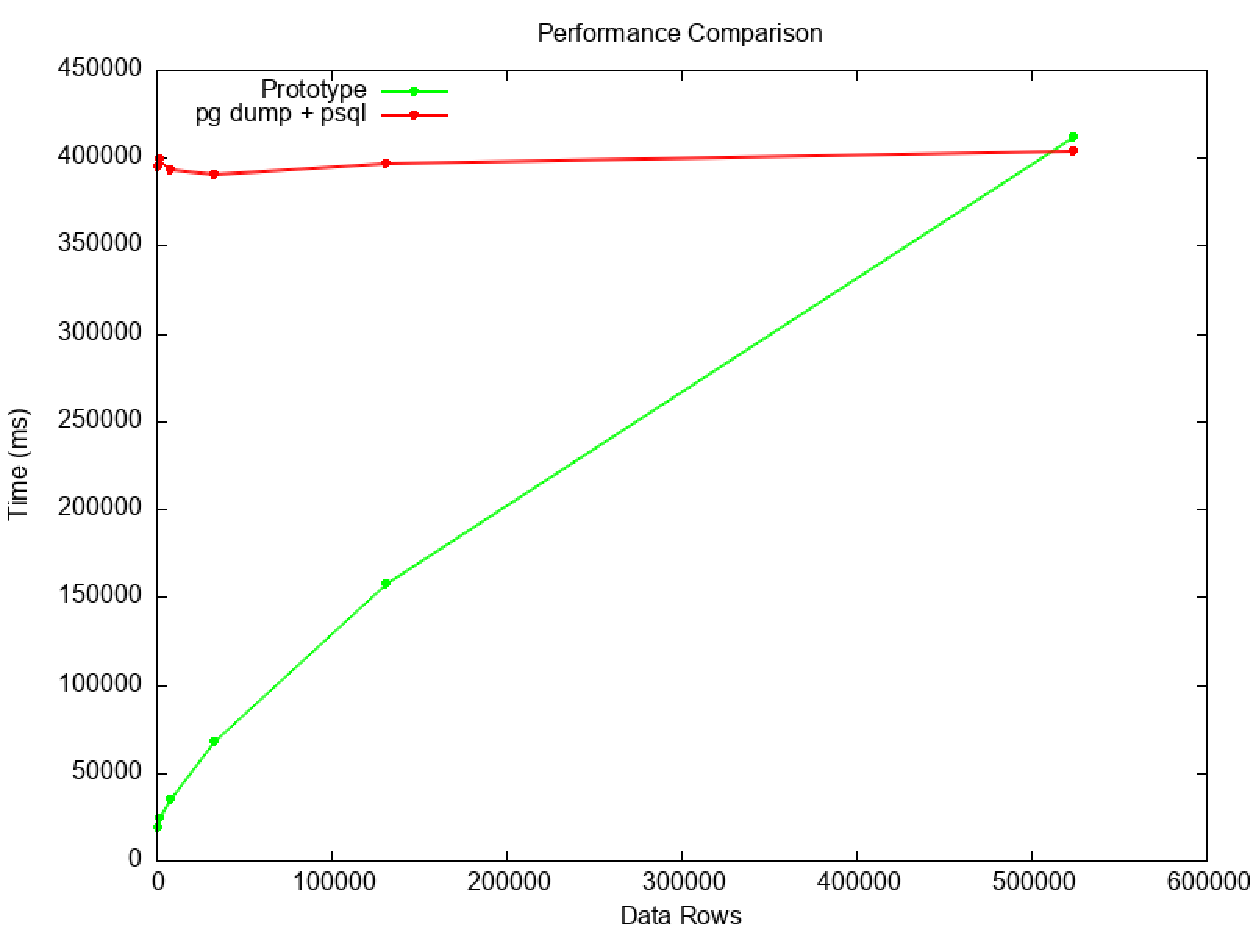
\includegraphics[height = 6cm]{img/benchmark}
	\end{center}
\end{frame}


\begin{frame}
\frametitle{Анализ результатов}
	\textbf{Результаты}:

	\begin{itemize}
		\item спроектирована общая архитектура;
		\item разработан язык описания обхода и трансформации данных;
		\item реализован минимально жизнеспособный продукт.
	\end{itemize}

	\textbf{Дальнейшие перспективы}:
	\begin{itemize}
		\item улучшение производительности;
		\item реализация механизмов анонимизации и генерации данных.
	\end{itemize}

\end{frame}


\begin{frame}
\frametitle{Описание программной разработки}
	Ссылки на код грамматики и код минимально жизнеспособного продукта

	\begin{center}
		
\includegraphics[height = 6cm]{img/qr-code-relatio-lang}
	\end{center}
\end{frame}


\begin{frame}
\frametitle{Приложения}
	Алгоритм генерации данных

	\begin{center}
		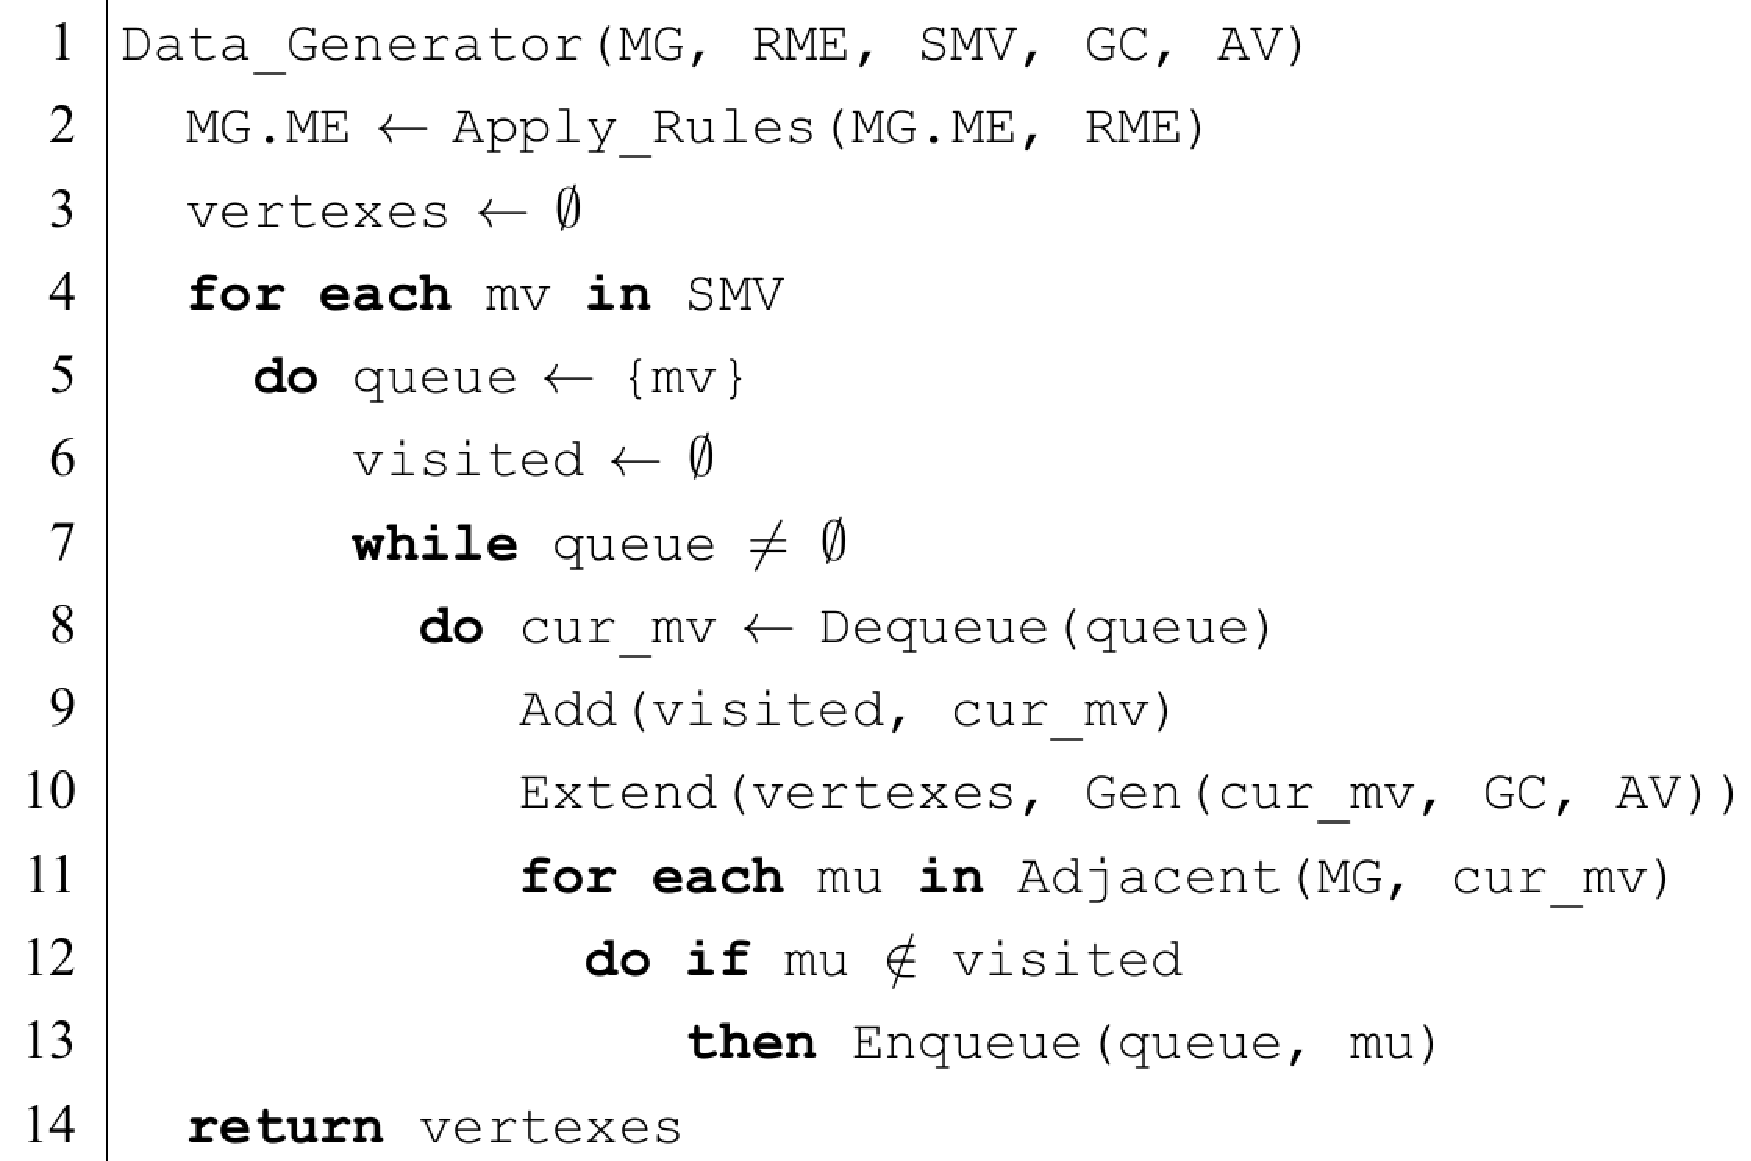
\includegraphics[height = 6cm]{img/extra-alg-generator}
	\end{center}
\end{frame}


\begin{frame}
\frametitle{Приложения}
	Архитектура на уровне контекста

	\begin{center}
		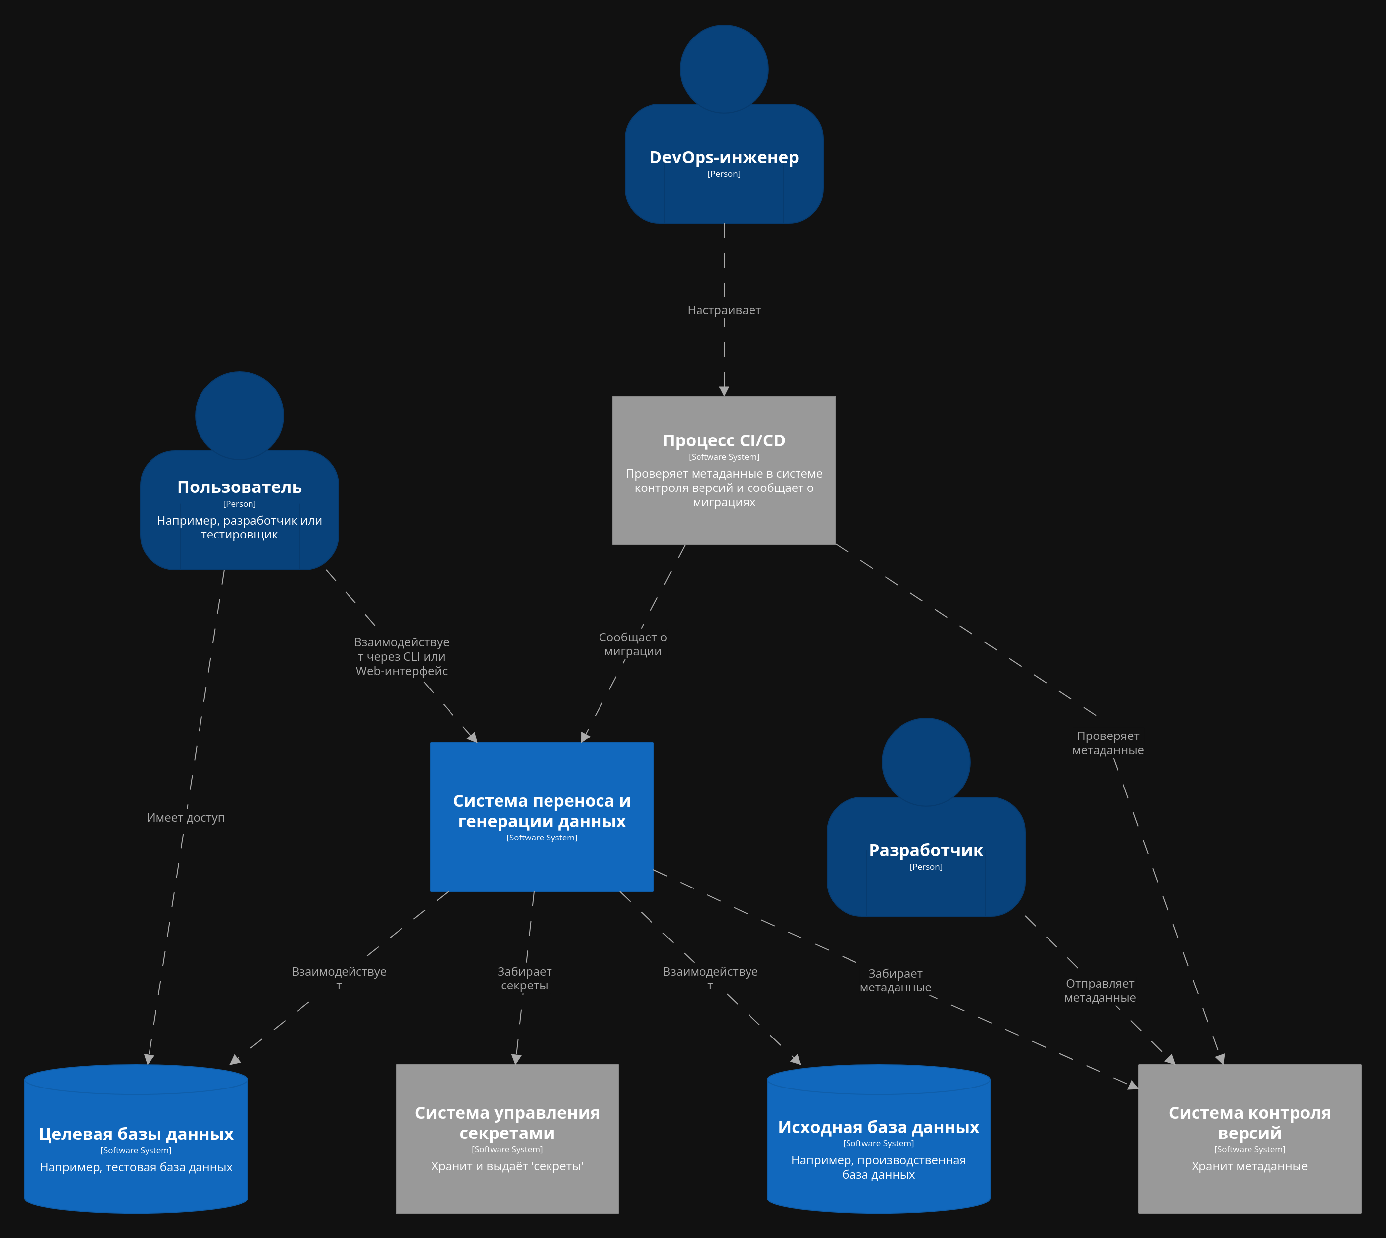
\includegraphics[height = 6cm]{img/structurizr-SystemLandscape}
	\end{center}
\end{frame}


\begin{frame}
\frametitle{Приложения}
	Архитектура на уровне контейнеров

	\begin{center}
		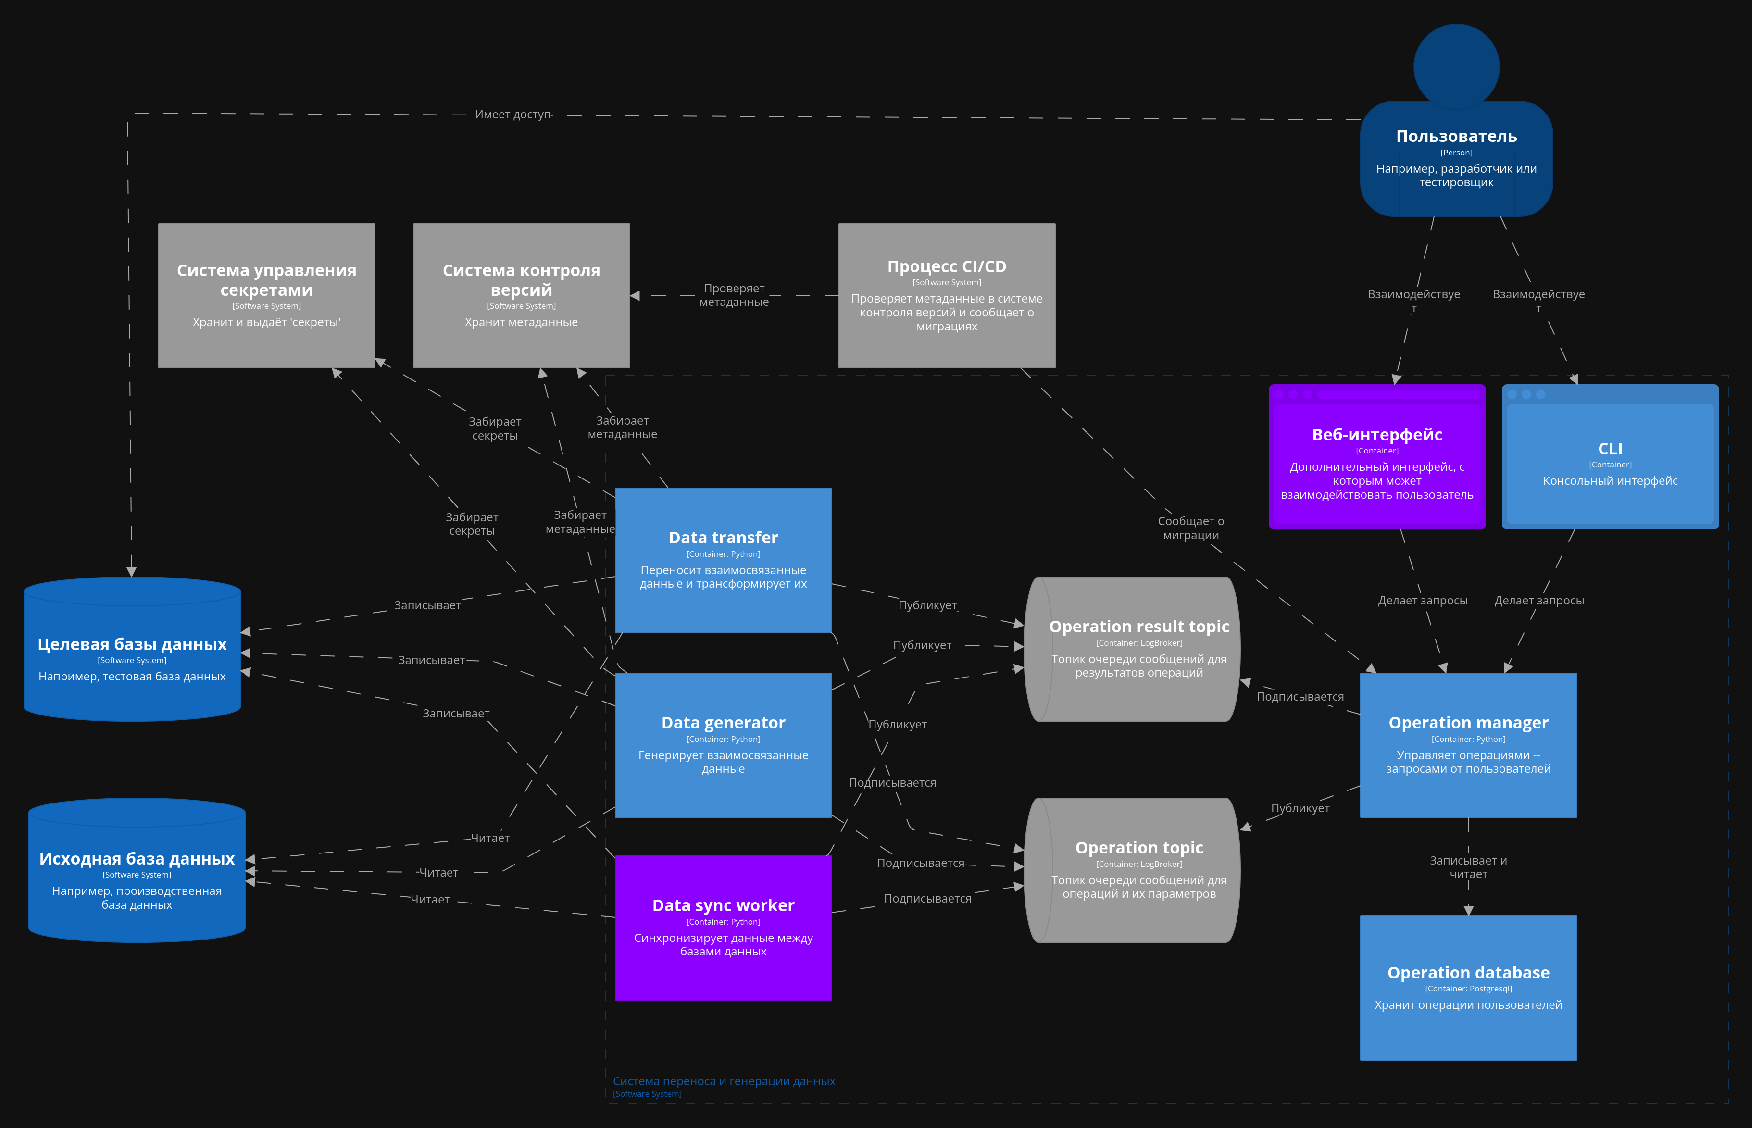
\includegraphics[height = 6cm]{img/structurizr-Containers}
	\end{center}
\end{frame}


\begin{frame}
\frametitle{Приложения}
	Архитектура на уровне компонент (Data Transfer)

	\begin{center}
		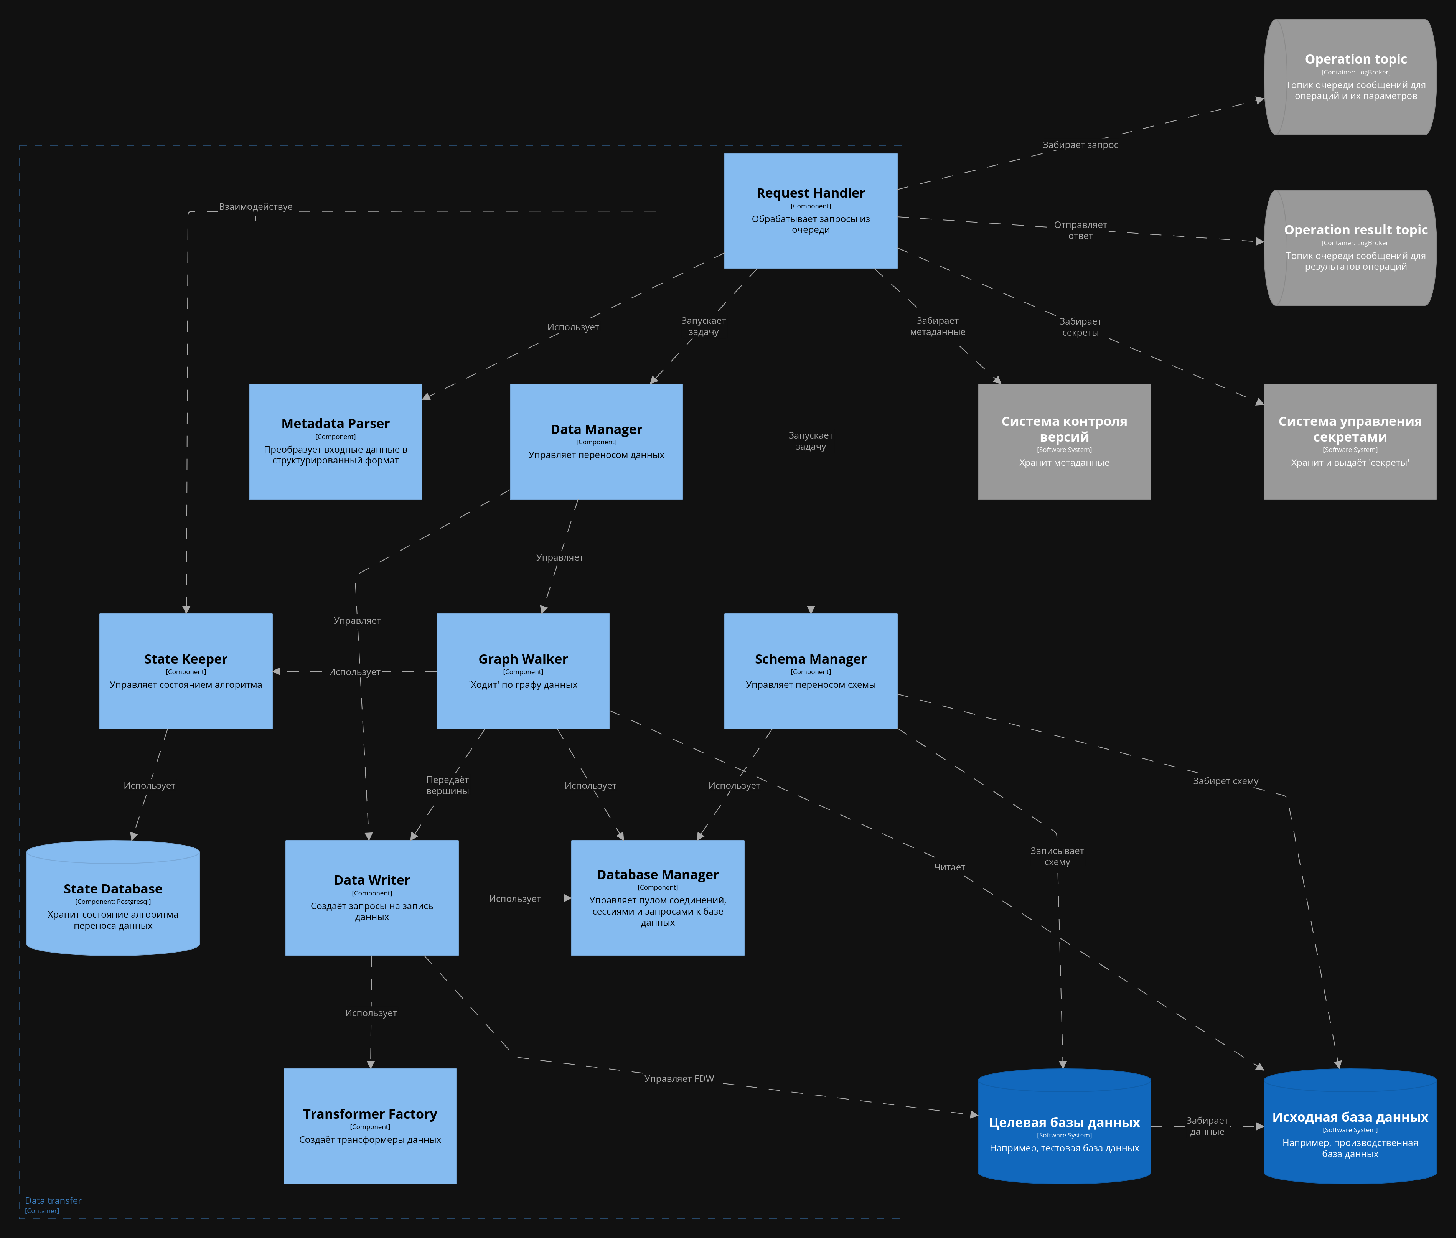
\includegraphics[height = 6cm]{img/structurizr-DataTransferComponents}
	\end{center}
\end{frame}
\end{document}
